\section{Experiments}\label{sec:experiments}
For our experiments we plan and execute queries for three separate survey-based data sets, showing that our system is well suited for early dataset exploration.
We show that \ProjectName{} performs an order of magnitude better than imputation on the full dataset and produces results of comparable quality.

\subsection{Implementation}
To evaluate the performance of our approach, we implemented a prototype system in Java, following a traditional iterator model.
Our database handles a subset of standard SQL queries, including filters, joins, projection, grouping and aggregation.
For simplicity, \ProjectName{} only handles tables containing integer data, so we pre-process our experimental datasets before loading them.

\subsection{Data sets}\label{subsec:datasets}
We collected three data sets for our experiments.
For all data sets, we selected a subset of the original attributes.
We also transformed all data values to an integer representation by enumerating strings and transforming floating-point values into an appropriate range.

\subsubsection{CDC NHANES}
For our first set of experiments, we use survey data collected by the 
Centers for Disease Control and Prevention (CDC) in the United States. We
experiment on a set of tables collected as part of the 2013--2014 National
Health and Nutrition Examination Survey (NHANES), a series of studies
conducted by the CDC on a national sample of several thousand individuals~\cite{cdc-data}.
The data consists on survey responses, physical examinations, and laboratory
results, amongst others.

There are 6 tables in the NHANES data set. We use three tables for our experiments:

\begin{itemize}
	\item \emph{Demographics}: demographic information of subjects
	\item \emph{Examinations}: physical exam results
	\item \emph{Laboratory}: laboratory exam results
\end{itemize}

The original tables have a large number of attributes, in some cases providing more granular tests results or alternative metrics.
We focused on a subset of the attributes for each table to simplify the presentation and exploration of queries.
\Cref{table:nhanes-description} shows the attributes selected, along with the percentage of \nullv{} values for each attribute.
For readability, we have replaced the NHANES variable names with self-explanatory attribute names.

\begin{table}
  \centering
  \begin{subtable}{0.5\textwidth}
    \centering
    \begin{tabular}{llr}
\toprule
\textbf{Attribute} &  \textbf{\% Missing} \\
\midrule
age\_months &      93.39 \\
age\_yrs &       0.00 \\
gender &       0.00 \\
id &       0.00 \\
income &       1.31 \\
is\_citizen &       0.04 \\
marital\_status &      43.30 \\
num\_people\_household &       0.00 \\
time\_in\_us &      81.25 \\
years\_edu\_children &      72.45 \\
\bottomrule
\end{tabular}

    \caption{Demographics. \demorows{} rows.}
  \end{subtable}
  \par\medskip
  \begin{subtable}{0.5\textwidth}
    \centering
    \begin{tabular}{lS[table-format=2.2]}
\toprule
\textbf{Attribute} &  \textbf{Missing} \\
\midrule
albumin &      17.95\ \% \\
blood\_lead &      46.86\ \% \\
blood\_selenium &      46.86\ \% \\
cholesterol &      22.31\ \% \\
creatine &      72.59\ \% \\
hematocrit &      12.93\ \% \\
id &       0.00\ \% \\
triglyceride &      67.94\ \% \\
vitamin\_b12 &      45.83\ \% \\
white\_blood\_cell\_ct &      12.93\ \% \\
\bottomrule
\end{tabular}

%%% Local Variables:
%%% mode: latex
%%% TeX-master: "../main"
%%% End:

    \caption{Laboratory Results. \labexrows{} rows.}
  \end{subtable}
  \par\medskip  
  \begin{subtable}{0.5\textwidth}
    \centering
    \begin{tabular}{llr}
\toprule
 Table &                Attribute &  \% Missing \\
\midrule
 exams &        arm\_circumference &       5.22 \\
 exams &      blood\_pressure\_secs &       3.11 \\
 exams &  blood\_pressure\_systolic &      26.91 \\
 exams &          body\_mass\_index &       7.72 \\
 exams &                cuff\_size &      23.14 \\
 exams &       head\_circumference &      97.67 \\
 exams &                   height &       7.60 \\
 exams &                       id &       0.00 \\
 exams &      waist\_circumference &      11.74 \\
 exams &                   weight &       0.92 \\
\bottomrule
\end{tabular}

    \caption{Physical Results. \labexrows{} rows.}
  \end{subtable}
  \par\medskip  
  \caption{Missing value distribution for each table/attribute in CDC NHANES 2013--2014 data.}\label{table:nhanes-description} 
\end{table}

\subsubsection{freeCodeCamp 2016 New Coder Survey}
For our second set of experiments, we use data collected by freeCodeCamp, an open-source
community for learning to code, as a part of a survey of new software
developers~\cite{fcc-data}.  The \textit{2016 New Coder Survey} consists of responses by
over 15,000 people to 48 different demographic and programming-related questions.  The
survey targeted users who were related to coding organizations.

We use a version of the data that has been pre-processed, but where missing values remain.
For example, 46.6\% of \textit{commutetime} responses are missing. However, it is worth
noting that some of the missing values are also expected, given the way the data has been
de-normalized. For example, \textit{bootcamploanyesno}, a binary attribute encoding whether
a respondent had a loan for a bootcamp, is expected to be \nullv{} for participants who did not
attend a bootcamp.

We choose a subset of 17 attributes, which are shown in~\Cref{table:fcc-description} along
with the percentage of missing values.

\begin{table}
  \centering
  \begin{tabular}{lr}
\toprule
            \textbf{Attribute} &  \textbf{\% Missing} \\
\midrule
age &      12.85 \\
attendedbootcamp &       1.54 \\
 bootcampfinish &      94.03 \\
 bootcampfulljobafter &      95.93 \\
 bootcamploanyesno &      94.02 \\
 bootcamppostsalary &      97.89 \\
childrennumber &      83.65 \\
citypopulation &      12.74 \\
commutetime &      46.61 \\
countrycitizen &      12.59 \\
gender &      12.00 \\
hourslearning &       4.34 \\
income &      53.08 \\
moneyforlearning &       6.02 \\
monthsprogramming &       3.88 \\
schooldegree &      12.43 \\
studentdebtowe &      77.50 \\
\bottomrule
\end{tabular}

  \caption{Missing value distribution for each attribute in freeCodeCamp Survey Data}\label{table:fcc-description} 
\end{table}

\subsubsection{American Community Survey}
For our final experiment, we run a simple aggregate query over data from the American
Community Survey (ACS), a comprehensive survey conducted by the U.S.
Census Bureau. We use a cleaned version of the 2012 Public Use Microdata Sample (PUMS)
data kindly provided by the authors of~\cite{akande2015empirical}. Given that the data had
been cleaned, we artificially dirtied it by replacing 40\% of the values uniformly at random with \nullv{} values.
The final dataset consists of 671,153 rows and 37 integer columns.

\subsection{Queries}
We collect a set of queries (\Cref{fig:queries}) that we think are interesting to plan.
We believe that they could reasonably be written by a user in the course of data analysis.

The queries on the CDC NHANES data consist not only of projections and selections, but also
interesting joins and aggregates. Our aim was to craft meaningful queries that would
provide performance figures relevant to practitioners using similar datasets.

Our first set of queries is on the CDC data (\Cref{fig:queries-cdc}).
\Cref{q1} calculates calculate the average cuff size for individuals based on their income data, with a constraint on height.
\Cref{q2} compares creatine levels for individuals with low, medium, and high incomes and above a certain weight.
\Cref{q3} extracts the average blood lead levels for children under 6 years of age.
\Cref{q4} calculates the average systolic blood pressure, by gender, for subjects with a body mass index indicating obesity. 
\Cref{q5} calculates the average waist circumference for subjects above a certain height and weight.

Our second set of queries is on the freeCodeCamp data (\Cref{fig:queries-fcc}).
\Cref{q6} calculates the average income for higher-income survey participants, grouped by their bootcamp attendance.
\Cref{q7} estimates the average commute time of women from the United States who participated.
\Cref{q8} calculates the average amount of student debt based on school degree for survey participants who have student debt.
\Cref{q9} joins the freeCodeCamp data with a reference table provided by the World Bank which summarizes GDP per-capita across various countries~\cite{worldbank-data}.
The query calculates the average GDP per-capita of countries with and without bootcamp participants over 18 years of age.

\begin{table*}
  \todo{query parameter scaling}
  \centering
  \begin{subtable}{\linewidth}
    \newcounter{queryno}
\begin{tabular}{cl}
\toprule
\# & \multicolumn{1}{c}{Query} \\
\midrule
1 & 
\begin{minipage}{6in}
\begin{lstlisting}[breaklines]
SELECT income, AVG(height)
FROM demo, exams
WHERE demo.id = exams.id
GROUP BY income;
\end{lstlisting}
\end{minipage}\refstepcounter{queryno} \label{q1} \\
2 & 
\begin{minipage}{6in}
\begin{lstlisting}[breaklines]
SELECT income, AVG(cholesterol)
FROM demo, exams, labs
WHERE demo.id = exams.id AND exams.id = labs.id AND
      income >= 13 AND income <= 15 AND weight >= 63
GROUP BY income;
\end{lstlisting}
\end{minipage}
\refstepcounter{queryno} \label{q2} \\
3 & 
\begin{minipage}{6in}
\begin{lstlisting}[breaklines]
SELECT MAX(blood_lead)
FROM demo, exams, labs
WHERE demo.id = labs.id AND labs.id = exams.id AND age_yrs <= 6;
\end{lstlisting}
\end{minipage}\refstepcounter{queryno} \label{q3}\\
4 & 
\begin{minipage}{6in}
\begin{lstlisting}[breaklines]
SELECT gender, AVG(blood_pressure_systolic)
FROM demo, labs, exams
WHERE demo.id = labs.id AND labs.id = exams.id AND
      body_mass_index >= 30
GROUP BY gender;
\end{lstlisting}
\end{minipage}\refstepcounter{queryno} \label{q4}\\
%5 & 
%\begin{minipage}{6in}
%\begin{lstlisting}[breaklines]
%SELECT age_yrs, gender, triglyceride, waist_circumference
%FROM demo, labs, exams
%WHERE demo.id = exams.id AND labs.id = exams.id AND
%      labs.triglyceride > 200;
%\end{lstlisting}
%\end{minipage}\refstepcounter{queryno} \label{q5}\\
\bottomrule
\end{tabular}

    \caption{Queries on CDC data}\label{fig:queries-cdc}
  \end{subtable}
  \par\medskip
  \begin{subtable}{\linewidth}
    \begin{tabular}{cl}
\toprule
\# & \multicolumn{1}{c}{Query} \\
\midrule
6 & 
\begin{minipage}{6in}
\begin{lstlisting}[breaklines]
SELECT attendedbootcamp, AVG(income)
FROM fcc
GROUP BY attendedbootcamp;
\end{lstlisting}
\end{minipage}\refstepcounter{queryno} \label{q6} \\
7 & 
\begin{minipage}{6in}
\begin{lstlisting}[breaklines]
SELECT AVG(age)
FROM fcc
WHERE gender = 178 AND countrycitizen = 158;
\end{lstlisting}
\end{minipage}\refstepcounter{queryno} \label{q7} \\
8 & 
\begin{minipage}{6in}
\begin{lstlisting}[breaklines]
SELECT schooldegree, AVG(moneyforlearning)
FROM fcc
WHERE studentdebtowe > 0 AND schooldegree >= 0
GROUP BY schooldegree;
\end{lstlisting}
\end{minipage}\refstepcounter{queryno} \label{q8}\\
9 & 
\begin{minipage}{6in}
\begin{lstlisting}[breaklines]
SELECT attendedbootcamp, AVG(gdp_per_capita)
FROM fcc, gdp
WHERE fcc.countrycitizen = gdp.country
GROUP BY attendedbootcamp;
\end{lstlisting}
\end{minipage}\refstepcounter{queryno} \label{q9}\\
10 & 
\begin{minipage}{6in}
\begin{lstlisting}[breaklines]
SELECT bootcamppostsalary, gdp_per_capita
FROM fcc, gdp
WHERE fcc.countrycitizen = gdp.country AND
      fcc.bootcamppostsalary <= 2 AND
      gdp.gdp_per_capita <= 5000;
\end{lstlisting}
\end{minipage}\refstepcounter{queryno} \label{q10}\\
\bottomrule
\end{tabular}

    \caption{Queries on freeCodeCamp data}\label{fig:queries-fcc}
  \end{subtable}
  \par\medskip
  \caption{Queries used in our experiments.}\label{fig:queries}
\end{table*}

%\begin{table*}
%  \centerfloat
%  \begin{tabular}{cSSSSSSS}
\toprule
\multicolumn{2}{c}{} & \multicolumn{2}{c}{Imputed ($\alpha=0.0$)} & \multicolumn{2}{c}{Imputed ($\alpha=1.0$)} \\
\cmidrule(r){3-4}
\cmidrule(l){5-6}
\# & \multicolumn{1}{c}{Base error} & \multicolumn{1}{c}{Error} & \multicolumn{1}{c}{Time (s)} & \multicolumn{1}{c}{Error} & \multicolumn{1}{c}{Time (s)} \\
\midrule
\ref{q1} & 5.25e+03 & 0.00e+00 & 1.723 & -3.60e+03 & 11.008 \\
\ref{q2} & 3.38e+04 & 0.00e+00 & 1.748 & -3.37e+04 & 10.144 \\
\ref{q3} & 9.32e-04 & 0.00e+00 & 1.732 & 2.54e-02 & 33.04 \\
\ref{q4} & 1.78e+05 & 0.00e+00 & 1.778 & -1.55e+05 & 21.013 \\
\ref{q5} & 9.89e-04 & 0.00e+00 & 1.712 & 9.89e-02 & 7.981 \\
\ref{q6} & 1.01e-02 & 0.00e+00 & 1.982 & 1.13e-02 & 52.309 \\
\ref{q7} & 0.00e+00 & 0.00e+00 & 43M49.786 & 0.00e+00 & 5.946 \\
\ref{q8} & 0.00e+00 & 0.00e+00 & 1.776 & 0.00e+00 & 3.172 \\
\ref{q9} & \multicolumn{1}{c}{--} & \multicolumn{1}{c}{--} & 1.919 & \multicolumn{1}{c}{--} & 2M40.384 \\
\ref{q10} & \multicolumn{1}{c}{--} & \multicolumn{1}{c}{--} & 0.01 & \multicolumn{1}{c}{--} & 7.786 \\
\ref{q11} & \multicolumn{1}{c}{--} & \multicolumn{1}{c}{--} & 0.007 & \multicolumn{1}{c}{--} & 0.103 \\
\ref{q12} & 0.00e+00 & 0.00e+00 & 0.008 & 1.00e-02 & 0.175 \\
\ref{q13} & \multicolumn{1}{c}{--} & \multicolumn{1}{c}{--} & 0.407 & \multicolumn{1}{c}{--} & 0.4 \\
\ref{q14} & 0.00e+00 & 0.00e+00 & 0.752 & 4.37e-01 & 1M14.221 \\
\bottomrule
\end{tabular}

%    \caption{Base error, percent change in error and and running time for queries
%    with different imputation levels. Base error is the root-mean-square error (RMSE) between the query on clean
%    data and the query run on dirty data without imputation. Change in error is relative to the base error.}
%  \label{fig:experiments}
%\end{table*}

All experiments were run on a single Amazon Web Services EC2 {\tt c4.xlarge} instance, with
four 2.9 GHz Intel Xeon E5--2666 v3 virtual CPUs and 7.5 GiB of main memory, on Debian Linux.

\subsection{Results}\label{sec:results}

\Cref{fig:runtimes} shows a summary of the performance results. We evaluated three different
configurations for each query. We compare \ProjectName{} optimizing for quality ($\alpha=0.0$),
\ProjectName{} optimizing for performance ($\alpha=1.0$), and imputing at the base tables followed
by executing the query traditionally. The quality-optimized queries are an order-of-magnitude
faster than imputing on the base tables. We can get another order-of-magnitude speedup when
optimizing for performance. This performance differential means it is feasible
to explore multiple imputations operations (including more expensive operators) when using
\ProjectName{}, in contrast to the traditional approach of base table imputation.

\begin{figure}
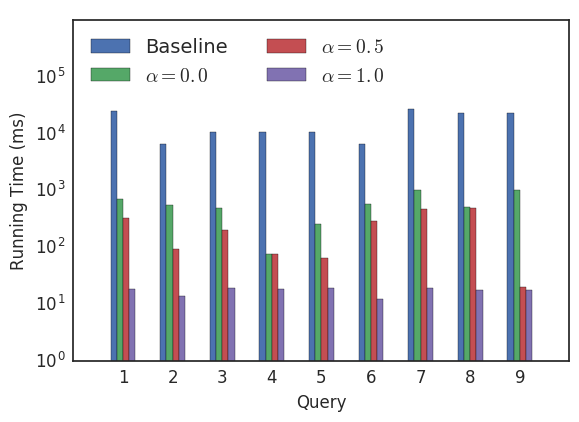
\includegraphics[width=\columnwidth]{figures/running_times_combined_bar.png}
\caption{Query runtimes with imputation on base tables, \ProjectName{}
    optimizing for quality ($\alpha=0$), and \ProjectName{} optimizing for
    performance ($\alpha=1$). Quality-optimized, on-the-fly imputation provides an order of
    magnitude speedup over imputing on base tables. Efficiency-optimized on-the-fly
    imputation can provide another order-of-magnitude speedup at the expense of quality.}
    
\label{fig:runtimes}
\end{figure}

%\Cref{fig:plantimes} provides a summary of the planning times for each of the queries.
%We exclude the planning time for queries that impute at base table, as that requires no
%planning. 

In the median query across a variety of queries and choices of $\alpha$, planning
constituted \planningruntimepercent{} percent of total runtime. In all cases, the optimizer
returned a query plan within \planningmaxtime{} ms, with times roughly constant between levels of $\alpha$.

% The one-standard-deviation
%intervals around the mean planning time often overlap, suggesting the planning component is
%constant in $\alpha$.

%\begin{figure}
%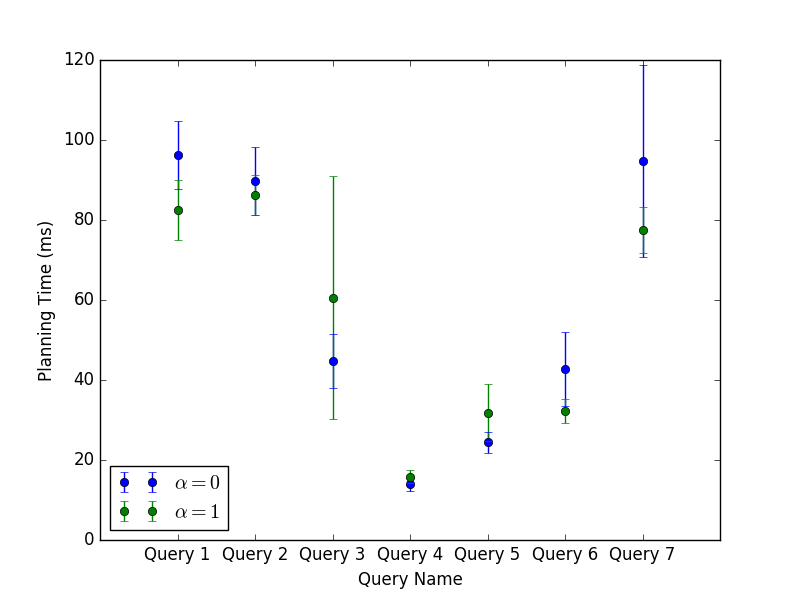
\includegraphics[width=\columnwidth]{figures/planning_times_imputedb.png}
%\caption{Planning times for each query}
%\label{fig:plantimes}
%\end{figure}

\subsubsection{Accuracy vs. Base-table Imputation}

\Cref{table:smape} shows the Symmetric-Mean-Absolute-Percentage-Error (SMAPE)~\cite{Makridakis2000451} for
\ProjectName{}'s query results when compared to the results of running imputation on the base tables and
executing the query on this cleaned base data \cite{tofallis2015better}. Given that the main datasets used
have no ground truth, this measure indicates how much error is introduced by on-the-fly imputation compared
to imputation on the base tables.

Each query was separately run 200 times in both settings and then results from the two approaches were
paired up and compared tuple-wise.  We average tuple-wise absolute percentage deviations
within each iteration of a query, and we report this value averaged over all iterations.  We
can see that optimizing for quality indeed reduces the SMAPE of query results.  In general, the SMAPE relative 
to the base-imputation approach is low in all cases---between
\lowsmapealphazero{} and \highsmapealphaoneexacs{} percent---indicating that on-the-fly
imputation produces similar results to imputation at the base tables.

We also calculate SMAPE over the number of tuples used to produce the results
in each configuration with respect to the number of tuples satisfying the same query when
the base tables have been imputed. In many cases where the SMAPE reduction between $\alpha = 1$ and
$\alpha = 0$ is small, for example \Cref{q6}\todo{confirm}, we highlight that the count of tuples can be significantly different between
the two scenarios. So while the aggregate used might not have been significantly affected by the different population,
other aggregates may well be. This highlights a challenge for a user handling data imputation traditionally: it is unclear if
the missing data will have a large or small negative impact on their analysis until they have paid the cost of
running it. By using \ProjectName{} this cost can be lowered significantly.


\begin{table}
\centering
\begin{tabular}{rrr}
\toprule
 Query &  \textbackslashalpha &  SMAPE \\
\midrule
     0 &     0.0 &   0.47 \\
     0 &     1.0 &   0.15 \\
     1 &     0.0 &   0.28 \\
     1 &     1.0 &   0.40 \\
     2 &     0.0 &   0.00 \\
     2 &     1.0 &   0.00 \\
     3 &     0.0 &   0.03 \\
     3 &     1.0 &   0.22 \\
     4 &     0.0 &  11.18 \\
     4 &     1.0 &    NaN \\
     5 &     0.0 &   0.79 \\
     5 &     1.0 &   1.93 \\
     6 &     0.0 &   0.00 \\
     6 &     1.0 &   0.03 \\
     7 &     0.0 &   0.82 \\
     7 &     1.0 &  35.44 \\
     8 &     0.0 &   0.23 \\
     8 &     1.0 &   0.31 \\
     9 &     0.0 & 100.00 \\
     9 &     1.0 & 100.00 \\
\bottomrule
\end{tabular}

\caption{Symmetric-Mean-Absolute-Percentage-Error for queries run under different $\alpha$
    parameterizations. To calculate SMAPE, \ProjectName{} results are compared to query results returned
    from executions with base table imputation. Queries optimized
    for quality ($\alpha=0$) generally achieve lower error than queries optimized for
    efficiency ($\alpha=1$). Count shares show the number of results returned from each
    query as a percentage of the number of results returned when imputing on the base table.
    A lower count share reflects more potential for errors.}
\label{table:smape}
\end{table}


\subsubsection{Runtime of Base-table Imputation}
In many real-world cases, applying the imputation step at the base table is prohibitively
expensive.
To illustrate the increasing difficulty of such an approach as datasets scale, we ran the following query over the ACS dataset:
\begin{lstlisting}[breaklines]
SELECT AVG(c0) FROM acs_dirty;
\end{lstlisting}
Applying the imputation operation to the base table is extremely expensive, as it imputes over all attributes in all rows, in our case
completing in \acsbaseresultminutes{}. In contrast, \ProjectName{} executes a quality-optimized version
in \acsimputedbzeroresult{} and a runtime-optimized version in \acsimputedboneresult{}. This highlights the potential
benefit of using our system for early data exploration. Note that the performance differential relative to base table imputation
would likely widen further if selection predicates were added to the query.

For every imputation inserted into the query plan, a new statistical model is instantiated and trained before being used for imputation.
Although it is tempting to further optimize query execution in \ProjectName{} by pre-training imputation models while the analyst begins to make queries,
this is not desirable because the specific rows of data, set of complete attributes, and set of attributes to impute are not known until runtime.

%\todobox{Jose: I'm not a fan of this line, I would remove}{Furthermore, at that point, it may make more sense to specify a coherent model over the entire base table instead.}

%%% Local Variables:

%%% mode: latex
%%% TeX-master: "main"
%%% End:
